\chapter{Arquitetura das Classes}
Neste capítulo falaremos do esqueleto da  aplicação UMeR, serão abordadas as classes presentes na aplicação assim como os atributos e funcionamento de cada uma e também as decisões tomadas.
\begin{figure}[htb]
	\centering
	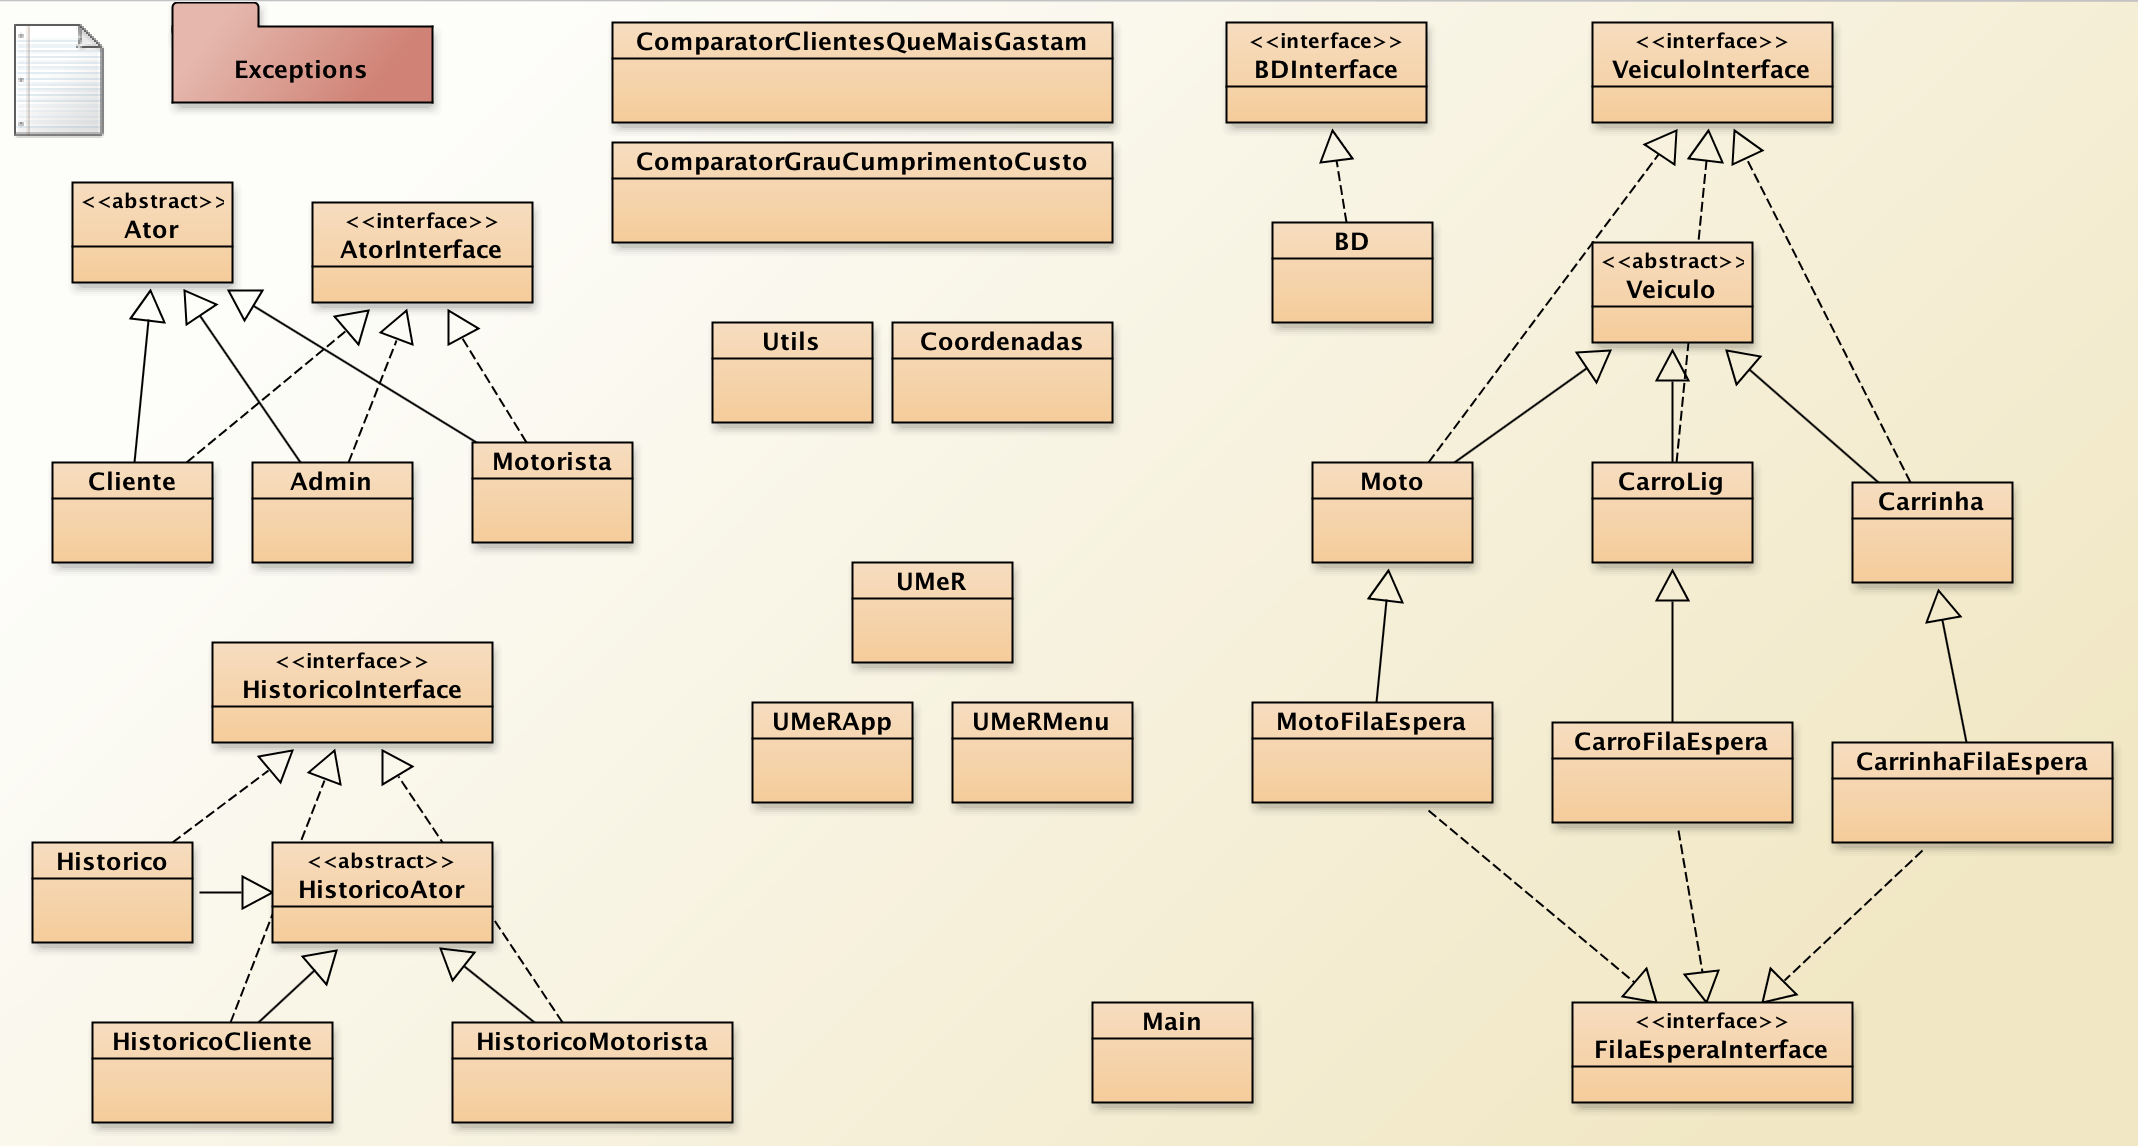
\includegraphics[scale=0.45]{imagem/esquemaClasses}
	\caption{Esquema de Classes do BlueJ }
	\label{p2:fig:p2_classes}
\end{figure}

\newpage

\section{AtorInterface}
A interface AtorInterface define todos os métodos que os utilizadores da aplicação deverão ter definidos. 
Se no futuro for pretendido adicionar novos tipos de atores ao sistema, essas classes deverão também elas implementar esta interface.  Desta forma poder-se-á inserir novos tipos de utilizadores à base de dados sem dificuldades. Como se pode visualizar na base de dados os utilizadores (motoristas, clientes e admins ) são coleções do tipo AtorInterface. Pode-se portanto adicionar os novos tipos de atores a cada uma destas coleções. 
 

\subsection{ Ator}
A classe  \textit{Ator} é uma classe abstrata e sevirá  como “modelo” para outras classes que dela herdem, não podendo ser instanciada por si só. Para ter um objeto de uma classe abstrata é necessário criar uma classe mais especializada que herda dela e então instanciar essa nova classe. Neste caso foram criadas as classes \textit{Admin}, \textit{Cliente} e  \textit{Motorista} que herdam a informação que está na classe superior (Ator).

\begin{figure}[htpb]
	\centering
	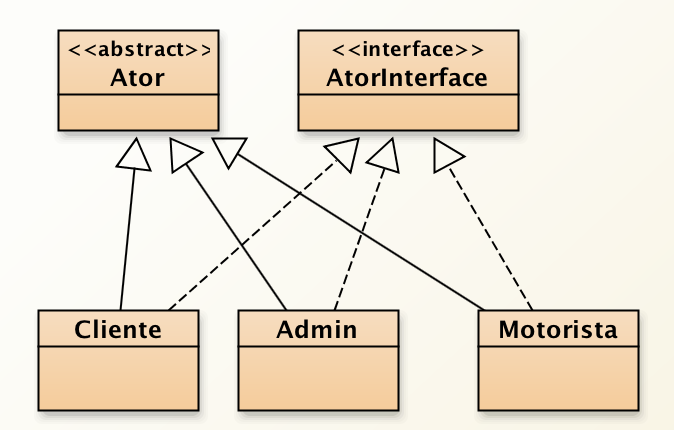
\includegraphics[scale=0.6]{imagem/atores}
	\caption{Classes }
	\label{p2:fig:p2_atoresr}
\end{figure}

As variáveis de instância da classe abstrata \textit{Ator} são apresentadas de seguida: 
\begin{verbatim}
private String email; 
private String nome; 
private String password; 
private String morada; 
private LocalDate dataNascimento; 
\end{verbatim}


\subsection{Admin}

Na classe \textit{Admin} estarão todos os dados herdados da classe \textit{Ator}. 


\subsection{Cliente}
Na classe \textit{Cliente} estarão todos os dados herdados da classe \textit{Ator}. 

\begin{verbatim}
private Coordenadas loc; //localização atual do cliente
private boolean emViagem;
\end{verbatim}
\subsection{Motorista}
Na classe \textit{Motorista} estarão todos os dados herdados da classe \textit{Ator}. 

\begin{verbatim}
private int grauCumprimentoHorario; //0-100
private int classificacao; //0-100
private double totalKms; 
private boolean disponivel;//verifica se está disponivel ou não 
private boolean horarioTrabalho; //verificar se está no horário de trabalho
private double destreza; //valor entre 0.5 e 1.9
private VeiculoInterface veiculo; 
private Historico viagemEmProcesso;
private int totalViagens;
\end{verbatim}

Decidimos que a destreza do motorista seria atribuida através da invocação de um random() que gera valores entre 0,5  e 1,9 afim de gerar alguma aleatoriedade nos tempos obtidos das viagens efetuadas. 
\begin{verbatim}
this.destreza = Utils.generateRandom(0.5f, 1.9f); 
\end{verbatim}

\newpage
\section{VeiculoInterface}

A interface VeiculoInterface define todos os métodos que os veiculos da aplicação deverão ter definidos. 
Se no futuro for pretendido adicionar novos tipos de veiculos ao sistema, essas classes deverão também elas implementar esta interface.  Desta forma poder-se-á inserir novos tipos de veiculosd à base de dados sem dificuldades. Como se pode visualizar na base de dados os veiculos (carros, motos, carrinhas, etc ) são coleções do tipo VeiculoInterface. Pode-se portanto adicionar os novos tipos de veiculos à coleção. 


\begin{figure}[htpb]
	\centering
	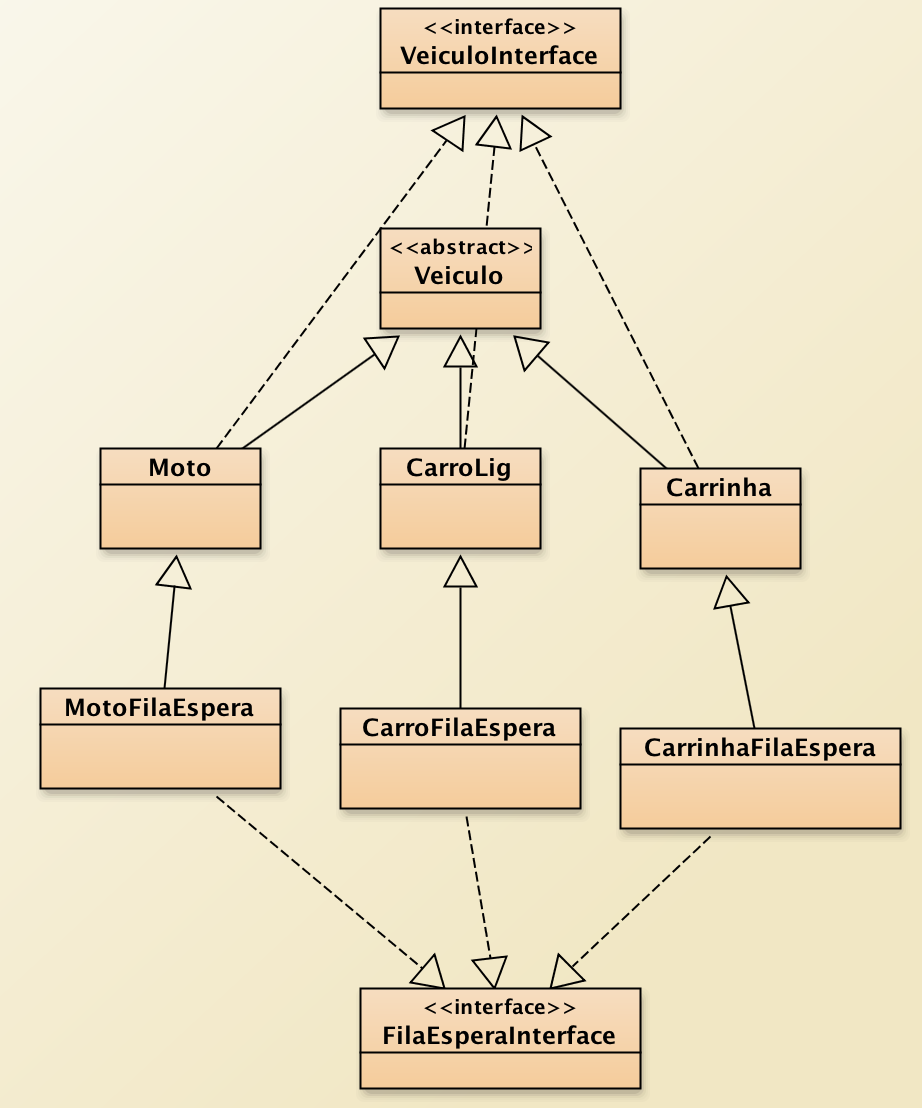
\includegraphics[scale=0.6]{imagem/veiculo}
	\caption{Classes }
	\label{p2:fig:p2_veiculos}
\end{figure}

\subsection{Veiculo}

\begin{verbatim}
private String matricula; 
private String marca; //Acrescentou-se a variável de instância marca, 
para o cliente poder escolher um carro com base na marca do veiculo

private float fiabilidade;//0 a 2 randon()
private Coordenadas loc;
\end{verbatim}

\section{Moto}
\begin{verbatim}
private static final int lugaresLivres = 1;
private static final double vm = 40.5; 
private static final double precoPorKm = 2.1;
\end{verbatim}

\subsection{MotoFilaEspera}
\begin{verbatim}
private List<Cliente> filaClientes;
\end{verbatim}

\section{CarroLig}

\begin{verbatim}
 private static final int lugaresLivres = 4;
private static final double vm = 65; 
private static final double precoPorKm = 3.5;
\end{verbatim}

\subsection{CarroFilaEspera}
\begin{verbatim}
private List<Cliente> filaClientes;
\end{verbatim}

\section{Carrinha}

\begin{verbatim}
private static int lugaresLivres = 8;
private static final double vm = 55;
private static final double precoPorKm = 5.1;
\end{verbatim}

\subsection{CarrinhaFilaEspera}
\begin{verbatim}
private List<Cliente> filaClientes;
\end{verbatim}

\newpage
\section{HistoricoInterface}
A interface HistoricoInterface define todos os métodos que os históricos da aplicação deverão ter definidos. 
Se no futuro for pretendido adicionar novos tipos de históricos ao sistema, essas classes deverão também elas implementar esta interface.  Desta forma poder-se-á inserir novos tipos de históricos à base de dados sem dificuldades. Como se pode visualizar na base de dados os históricos são coleções do tipo HistoricoInterface. Pode-se portanto adicionar os novos tipos de históricos à coleção. 

\subsection{Historico}
\begin{figure}[htpb]
	\centering
	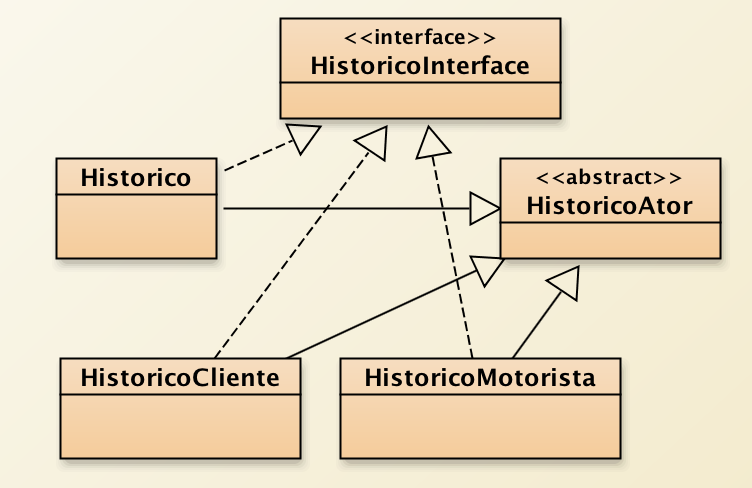
\includegraphics[scale=0.6]{imagem/historico}
	\caption{Classes }
	\label{p2:fig:p2_historico}
\end{figure}
\begin{verbatim}
private String emailCliente; 
private String emailMotorista; 
private LocalDateTime dataDeInicioDeServico;
private double distancia;
private double tempoEstimado; 
private double tempoReal;
private double valorEstimado; 
private double valorCobrado; 
private String estadoTempo;
private String estadoTransito; 
private boolean terminado; 
private Coordenadas origem;
private Coordenadas destino;
private int classificacao;
\end{verbatim}

\section{Utils}
Adicionalmente a classe \textit{Utils} tem implementado um método que encripta a password. E um método que gera números random com intervalos de 0.1. 

\subsection{Meteorologia}

Esta classe é usada para gerar fatores de aleatoriedade no cálculo real do tempo de viagem.

\begin{verbatim}
public static final String sol = "Sol"; 
public static final String nevoeiro  = "Nevoeiro"; 
public static final String granizo = "Granizo";
public static final String chuva = "Chuva";
public static final String neve = "Neve"; 
\end{verbatim}

\subsection{Trânsito}

Esta classe é usada para gerar fatores de aleatoriedade no cálculo real do tempo de viagem.

\begin{verbatim}
public static final String st = "Sem Transito"; 
public static final String tn = "Transito Normal"; 
public static final String mt  = "Muito Transito"; 
\end{verbatim}

\section{Coordenadas}

Esta classe guarda a localização de um utilizador. O construtor vazio está a ser usado na aplicação para gerar localizações aleatórias quando se criam os utilizadores. 

\begin{verbatim}
private double x;
private double y;
\end{verbatim}

As cordenadas também são iniciadas com o método random(). 
\begin{verbatim}
this.x=Utils.generateRandom(0f, 100f);
this.y=Utils.generateRandom(0f, 100f);
\end{verbatim}

O método getDistancia() calcula a distancia euclidiana, este será um método importante na execução da simulação de uma viagem. 
\begin{verbatim}
public double getDistancia (Coordenadas c){
    double distancia=0; 
    distancia = Math.sqrt( Math.pow((this.x - c.getX()),2 ) +
                           Math.pow((this.y - c.getY()),2 ));
    return distancia; 
}
\end{verbatim}

\section{BDInterface}
A interface BDInterface define todos os métodos que as classes que geram dados da aplicação deverão ter definidos. 

Se no futuro se pretender guardar a informação numa base de dados (Oracle por exemplo), esta classe deverá implementar a BDInterface. Desta forma, a mudança de classes que geram os dados guardados é muito simples uma vez que o resto da aplicação continuará a usar os mesmos métodos(definidos na BDInterface) que usa neste momento independentemente da forma como a classe implementa os métodos definidos pela interface. 

\subsection{BD}

As coleções clientes, motoristas e admins são do tipo Map e estão organizados pela chave que é o respetivo email. Uma vez que se efetuam muitas pesquisas, sobre estes dados com a chave email, a melhor opção seria um HashMap uma vez que a pesquisa pela chave é instântanea. 

Para a coleção de veiculos foi utilizada também um HashMap em que a chave é a matricula e os motivos são os mesmso descritos em cima.  Apesar de neste momento não se efetuar muitas pesquisas pela chave, imagina-se que no futuro tal poderá acontecer. 

A colecção de históricos escolhida foi o Set, pois não devem ser permitidos históricos repetidos. Uma vez que algumas das funcionalidades da aplicação implicavam percorrer os dados por ordem (data), pareceu-nos indicado usar um TreeSet e desta forma ter os dados guardados e ordenados de forma a facilitar as funcionalidade do programa.  

\begin{verbatim}
private Map<String, AtorInterface> clientes;
private Map<String, AtorInterface> motoristas; 
private Map<String, AtorInterface> admins; 
private Map<String,VeiculoInterface> veiculos; 
private Set<Historico> historico;
\end{verbatim}

\section{UMeRMenu}

Esta classe tem como objetivo facilitar a criação de menus e a leitura da opção introduzida. 

\begin{verbatim}
private String titulo;
private List<String> opcoes;
private int op;
\end{verbatim}

\section{UMeR}

Esta classe é o coração da aplicação, uma vez que é nela que está centralizada a lógica das gestão de viagens. É nesta classe que estão definidos os métodos para o calculo do tempo real, estimado, custo real e estimado, bem como métodos para devolver o motorista mais perto e estatisticas da aplicação. Sempre que necessário a UMeR delega a gestão dos dados(ler, guardar, atualizar, apagar) na classe da base de dados (BDInterface). 
Após login efetuado com sucesso a variável de instância atorloggado é inicializada com o utilizador que acabou de iniciar sessão. É com base nesta variável que a interface da aplicação(UMeRApp) decide quais os menus a apresentar.  

\begin{verbatim}
private BDInterface baseDeDados;
private AtorInterface atorLoggado;
private int tentativasDeLoginFalhadas;
\end{verbatim}

\section{UMeRApp}

Esta classe é responsável pela interface da aplicação. 

\begin{verbatim}
private static UMeR umer;
private static UMeRMenu menu_principal;
private static UMeRMenu menu_registar_atores;
private static UMeRMenu menu_motorista;
private static UMeRMenu menu_cliente;
private static UMeRMenu menu_dados_pessoais;
private static UMeRMenu menu_cliente_efetuarViagem;
private static UMeRMenu menu_admin;
private static UMeRMenu menu_registar_veiculos;
private static UMeRMenu menu_solicitarViagem; 
private static UMeRMenu menu_inserir_coord_destino;
private static UMeRMenu menu_terminar_viagem; 
private static UMeRMenu menu_terminar_horario_trabalho;
private static UMeRMenu menu_iniciar_horario_trabalho;
private static UMeRMenu menu_proposta_viagem;
private static UMeRMenu menu_historico;
\end{verbatim}




